% Each row is one recorded contact; all image pixels come from the supplied draft.
% The full-set reference is visually separated because it uses extra real supervision.
\definecolor{RendererReference}{RGB}{240,241,242}
\definecolor{RendererReferenceText}{RGB}{72,78,84}
\begin{tikzpicture}[x=1bp,y=-1bp]
\useasboundingbox (0,0) rectangle (248.4,121.5);
\fill[RendererReference] (198.5,0) rectangle (248.4,121.5);
\node[anchor=north west,inner sep=0pt] at (0,19.5)
  {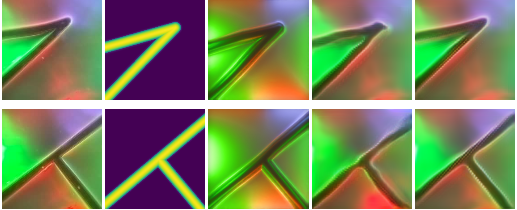
\includegraphics[width=248.4bp]{figures/src/renderer_image_grid.pdf}};
\node[anchor=north,inner sep=0pt,font=\fontsize{6.8bp}{8bp}\selectfont] at (25.08,7) {Real image};
\node[anchor=north,inner sep=0pt,font=\fontsize{6.8bp}{8bp}\selectfont] at (74.64,7) {GT depth};
\node[anchor=north,inner sep=0pt,font=\fontsize{6.8bp}{8bp}\selectfont] at (124.2,7) {PBR};
\node[anchor=north,inner sep=0pt,font=\fontsize{6.8bp}{8bp}\selectfont] at (173.76,7) {Learned $K{=}25$};
\node[anchor=north,inner sep=0pt,text=RendererReferenceText,font=\fontsize{6.8bp}{8bp}\selectfont] at (223.32,7) {Full set$^{\dagger}$};
\draw[RendererReferenceText,dashed,line width=0.35bp] (198.5,0) -- (198.5,121.5);
\end{tikzpicture}
